% 2010 年重庆卷理科第 20 题：双曲线 C（中心 O，右焦点 F）与两条渐近线、直线 l1、l2、MN 的位置图。
% 来源 PDF：普通高考/2010/2010重庆理.pdf，SHA-256 e981a8805207e307d0ec0d8ef50ac0e0cbf93eec9559a29fb88591b483ae0136。
% 原页：第 2 页（A3 三栏）第 2 栏中部，书页码 578。
% 重绘依据：按原页矢量路径换算成以 a=2 为单位的坐标（每单位 14.4 pt）：
%   原点 O(0,0)；x 轴 -1.97～6.64，y 轴 -3.93～3.69；
%   双曲线只画右支 x=2√(1+y²)（原页即只画右支，线较粗）；
%   两条渐近线均自 O 向右上方、右下方画出（原页也不画左半段）；
%   l1 过 M(-0.64,-0.98)，l2 过 N(1.69,0.42)，二者交于 E(5.3,-2.46)（在右支上）；
%   MN 过 M、N，与 y=x/2 交于 G(5.96,2.99)、与 y=-x/2 交于 H(0.54,-0.27)；
%   M、N 在原页为实心圆点，E、G、H 无圆点。
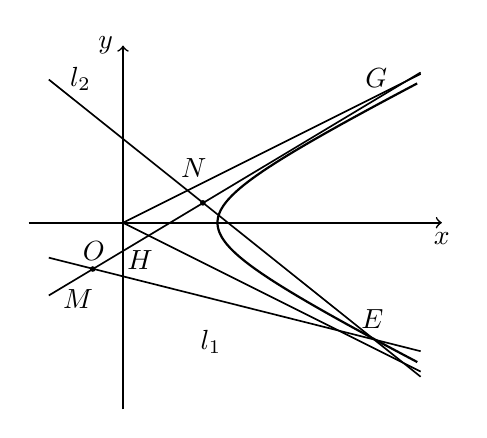
\begin{tikzpicture}[scale=0.6, semithick]
  \coordinate (O) at (0,0);
  \coordinate (M) at (-0.64,-0.98);
  \coordinate (N) at (1.69,0.42);
  \coordinate (E) at (5.30,-2.46);
  \coordinate (G) at (5.96,2.99);
  \coordinate (H) at (0.54,-0.27);

  % 坐标轴
  \draw[->] (-2.0,0) -- (6.75,0) node[below] {$x$};
  \draw[->] (0,-3.95) -- (0,3.75) node[left] {$y$};

  % 双曲线右支 x^2/4-y^2=1
  \draw[thick] plot[domain=-2.95:2.95, samples=140, variable=\y]
    ({2*sqrt(1+\y*\y)}, \y);

  % 渐近线 y=±x/2（只画右半）
  \draw (O) -- (6.30,3.15);
  \draw (O) -- (6.30,-3.15);

  % l1（过 M）、l2（过 N）、MN
  \draw (-1.57,-0.74) -- (6.30,-2.72);
  \draw (-1.57,3.03) -- (6.30,-3.26);
  \draw (-1.57,-1.54) -- (6.30,3.18);

  % 点 M、N 处实心圆点
  \fill (M) circle (1.7pt);
  \fill (N) circle (1.7pt);

  % 文字（位置照原页）
  \node at (-0.90,3.05) {$l_2$};
  \node at (1.86,-2.52) {$l_1$};
  \node at (-0.62,-0.60) {$O$};
  \node at (-0.95,-1.62) {$M$};
  \node at (1.50,1.16) {$N$};
  \node at (5.28,-2.03) {$E$};
  \node at (5.36,3.06) {$G$};
  \node at (0.36,-0.80) {$H$};
\end{tikzpicture}
